\documentclass[12pt]{article}
\usepackage{../../../lecture_notes}
\usepackage{../../../math}
\usepackage{../../../uark_colors}

\hypersetup{
  colorlinks = true,
  allcolors = ozark_mountains,
  breaklinks = true,
  bookmarksopen = true
}

\newcommand{\answer}[1]{{\color{blue_winged_teal}\textbf{Answer:} #1}}
\newcommand{\pts}[1]{{\color{zinc500}(#1 pts)}}

\begin{document}
\begin{center}
  {\Huge\bf Midterm 2 - Fall 2024}
  
  \smallskip
  {\large\it  ECON 4753 — University of Arkansas}
\end{center}

\vspace{5mm}
\begin{enumerate}
  \item \pts{10} Say you have the following time-series observations from $t = 1, \dots, 7$:
  \vspace*{-\bigskipamount}
  $$
    0.63, 0.79, 0.93, 1.1, 1.05, 1.2, 1.3
  $$

  \begin{enumerate}
    \item What is the 1-lag autocorrelation coefficient, $\hat{\rho}_1$?
    
    \answer{
      The sample mean equals 1.

      The variance is
      \begin{align*}
        \frac{1}{7 - 1} &\big( 
        (0.63 - 1)^2 + (0.79 - 1)^2 + (0.93 - 1)^2 + \\
        &(1.1 - 1)^2 + (1.05 - 1)^2 + (1.2 - 1)^2 + (1.3 - 1)^2 \big) \\
        &= 0.0547
      \end{align*}

      The autocovariance is given by 
      \begin{align*}
        \frac{1}{6} &\big( 
        (0.63 - 1) (0.79 - 1) + (0.79 - 1) (0.93 - 1) + (0.93 - 1) (1.1 - 1) + \\
        &(1.1 - 1) (1.05 - 1) + (1.05 - 1) (1.2 - 1) + (1.2 - 1) (1.3 - 1) \big) \\
        &= 0.0267
      \end{align*}

      Finally, the autocorrelation is $0.0267 / 0.0547 = 0.488$.
    }
      
    \item By hand, forecast into period $8$ using a one-sided 3-period rolling average.

    \answer{
      $$
        \hat{y}_{8} = \frac{1}{3} (1.05 + 1.2 + 1.3) = 1.183
      $$
    }
  \end{enumerate}
  
  \item \pts{10} Say you are working at a company with time-series data and you want to use some smoothing method for analyzing the patterns. 
  \begin{enumerate}
    \item Say you use a two-sided moving average. Your boss asks why you do not have a value of $\hat{y}_t$ on the ends of the time-series. Please explain why
    
    \answer{
      A two-sided moving average uses observations in the future and in the past to form the forecast. At the ends of our time-series we do not have enough observations in the past or in the future, so we can not form the average.
    }
    
    \item Your boss replies that they really want to predict into next month. How would you adjust your choice of smoothing method to do this?
    
    \answer{
      Instead, I would use either a one-sided moving average or a simple exponential smoothing to form my forecast. 
      Since these only use past observations, I can forecast into the future period. 
    }
  \end{enumerate}

  \item \pts{10} Say you are trying to forecast a time-series data into the future. You notice that there is a non-linear trend in the data. Explain in 1, maybe 2, sentences why you should not try to model this using higher-order polynomial terms
  
  \answer{
    Polynomials shoot off to $\pm \infty$ and so they can be unstable. This is especially true as I extrapolate outwards in the time-series.
  }
\end{enumerate}

\bigskip\bigskip
\noindent For the following questions, we will look at monthly US data on the median sales price of housing (see Figure 1). In addition to the raw data, Figure 1 plots the estimated linear trend.

\begin{enumerate}
  \setcounter{enumi}{3}
  \item \pts{15} Consider a simple exponential smoothing model for inference on this time-series with $\alpha = 0.1$. For this time-series, how do you think this method would perform? Please explain why.
  
  \answer{
    This method would perform poorly. 
    With $\alpha = 0.1$, this imposes a lot of smoothing on the model and hence it would likely miss the short-term peaks and valleys we see between 2019 and 2023. 
    Moreover, since the data is trending, it will fail to capture these trends.
  }
  
  \item \pts{10} How do you think the linear time trend performs at describing this time series? What might you do to improve this time-series model?
  
  \answer{
    The linear time trend does an okay job; it picks up on the general growth of housing prices, but does not capture the intense growth starting in 2020.
    I might modify this by using a piecewise trends model.
  }
\end{enumerate}


\noindent For the following questions, we will be looking at daily time-series on taxis in NYC (see Figure 2). The outcome variable is the number of taxis out at noon each day. I have highlighted on the plot the days around Christmas where a large number of people typically leave the city.

Use the results of the follwoing time-series regression to answer the following questions
\begin{codeblock}[{}]
OLS estimation, Dep. Var.: n_taxis_at_noon
Observations: 140
Standard-errors: Heteroskedasticity-robust 
                  Estimate Std. Error  t value   Pr(>|t|)    
(Intercept)      19857.05    496.397 40.00235  < 2.2e-16 ***
day_of_week::Mon -3319.15    530.684 -6.25447 5.0606e-09 ***
day_of_week::Tue -2357.85    543.931 -4.33483 2.8561e-05 ***
day_of_week::Wed -1677.25    532.226 -3.15139 2.0080e-03 ** 
day_of_week::Thu -2176.00    729.170 -2.98422 3.3840e-03 ** 
day_of_week::Fri -1939.30    594.769 -3.26059 1.4122e-03 ** 
day_of_week::Sat  1343.60    751.638  1.78756 7.6124e-02 .   
---
Signif. codes:  0 '***' 0.001 '**' 0.01 '*' 0.05 '.' 0.1 ' ' 1
\end{codeblock}

\begin{enumerate}
  \setcounter{enumi}{5}
  \item \pts{10} What is the omitted category in this regression?
  
  \answer{The omitted category is Sunday.}
  
  \item \pts{10} Which day of the week has the most taxis available? 
  
  \answer{The day with the most taxis available is Saturday since it has the largest coefficient estimate and is positive (relative to Sunday).}

  \item \pts{15} Form a 95\% confidence interval for the average number of taxis available at noon on Sunday (round your answer to the nearest whole unit)
  
  \answer{With 95\% confidence, the number of taxis available at noon on Sundays is $19857 \pm 1.96 * 496.39 = (18884, 20829)$.}
    
  \item \pts{10} Do you think an adjustment should be made in the regression for the fact that the number of taxis has a sizeable drop around Christmas/New Years? What adjustment could you make?
  
  \answer{I would include an indicator variable in my time-series regression for being in the interval of dates highlighted by the gray bar.}
\end{enumerate}


\begin{figure}[ht!]
  \caption{Median Housing Price of Monthly US Sales}
  \label{fig:housing}
  
  \vspace*{-\bigskipamount}
  \begin{center}
    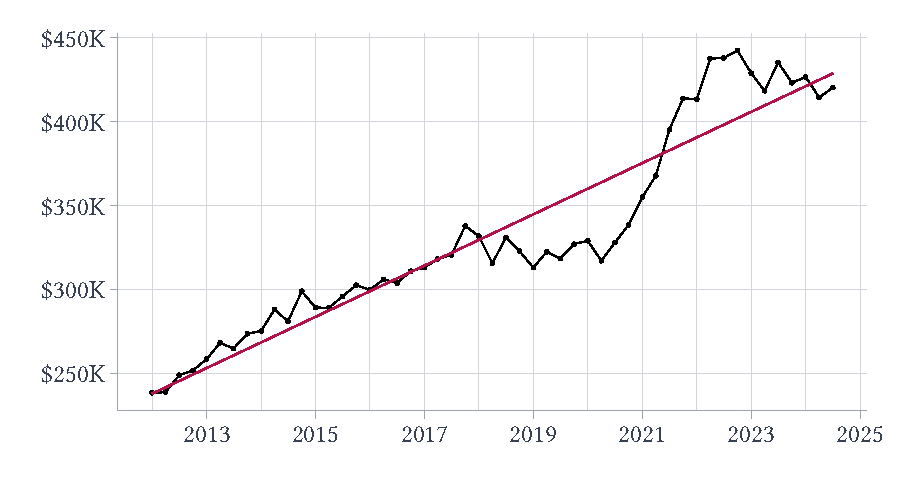
\includegraphics[width = 0.9\textwidth]{figures/median_us_housing_price_raw.pdf}
  \end{center}
\end{figure}

\begin{figure}[ht!]
  \caption{Daily data on the Number of Taxis available at Noon in NYC}
  \label{fig:taxi}

  \vspace*{-\bigskipamount}
  \begin{center}
    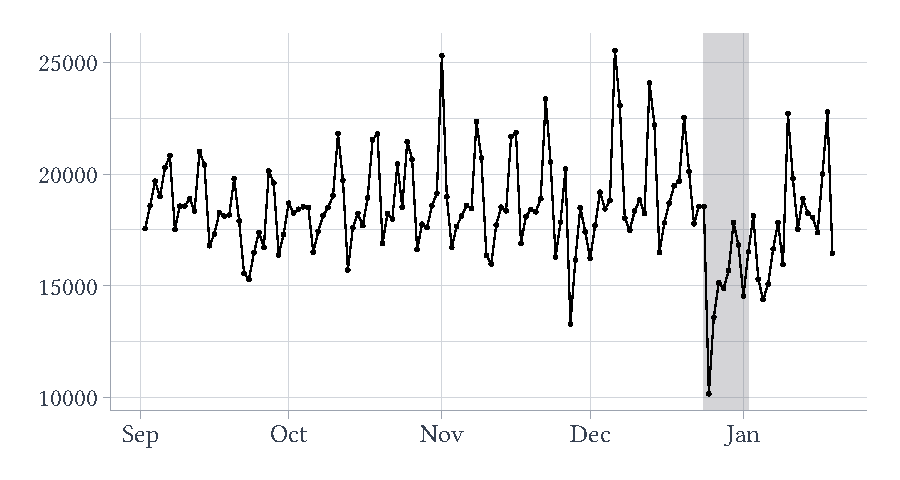
\includegraphics[width = 0.9\textwidth]{figures/nyc_taxis_raw.pdf}
  \end{center}
\end{figure}



\end{document}
